\documentclass[%
  manuscript=article,   % Use a - if you need a space e.g.,
  year=2024,
  volume=77,
  doi=00000.000,
%  recvd=November 18, 2024,
%  revd=January 30, 2025,
%  accptd=2025-02-11,
]{zfn}

\usepackage{amsmath}
\usepackage[nopatch]{microtype}
\usepackage{booktabs}

\usepackage{hyperref}
\hypersetup{colorlinks=true, linkcolor=black, citecolor=black, urlcolor=black, breaklinks=true, linktocpage}




%%%%%%%%%%%%%%%%%%%%%%%%%%%%%%%%%%%%%%%%%%%%%%%%%%%%%%%%%%%

	
\title{Explaining the undecidability of first-order logic}

\author{Timm Lampert}
\affiliation{FernUniversität Hagen}
\email[Timm Lampert]{lampertt@staff.hu-berlin.de}

\author{Anderson Nakano}
\affiliation{Pontifícia Universidade Católica São Paulo}
% \alsoaffiliation{Joint first authors}

%\author{T. Author}
%\affiliation{Second Division, Organization, City, Pincode, State, Country}
%
%\author{F.T. Author}
%\affiliation{Fourth Division, Organization, City, Pincode, State, Country}



\addbibresource{Lampert_PU.bib}

\keywords{constructive proof, automated theorem proving, Entscheidungsproblem, pattern detection, halting problem} %% First letter not capped

\begin{document}

\begin{abstract}
Turing proved the unsolvability of the decision problem for first-order logic (\emph{Entscheidungsproblem}) in his famous paper \emph{On Computable Numbers, with an Application to the Entscheidungsproblem}. From this proof it follows that attempts to specify a solution for the \emph{Entscheidungsproblem} through pattern detection in automated theorem proving (ATP) must fail. Turing's proof, however, merely predicts the non-existence of such solutions; it does not construct concrete examples that explain why specific attempts to solve the decision problem by pattern detection fail. ATP-search often runs in infinite loops in the case of unprovable, i.e. not refutable, formulas and one can ask why finite patterns of repeated inference steps cannot serve as criteria for unprovability.   
We answer this question by constructing pairs of formulas $(\phi,\phi')$ such that $\phi$ is provable (refutable) and $\phi'$ is unprovable (satisfiable in an infinite domain) but all but the last proof step of the ATP-search for $\phi$ is a proper part of the endless ATP-search for $\phi'$.
We generate such pairs of formulas by mimicking computable sequences for a certain kind of universal Turing machine, namely, splitting Turing machines (STMs), via sequences of inference steps in ATP. In contrast to Turing's and the textbooks' method to formalize Turing machines, our method does not rely on further axioms and allows us to transfer the straightforward insight that the halting problem cannot be solved through pattern detection to the case of the \textit{Entscheidungsproblem}. Our method is a constructive alternative to general undecidability proofs that explains why a scientific problem, namely the \emph{Entscheidungsproblem}, is unsolvable in a specific way.
This explanation provides a better understanding of the failure of pattern detection, which is of interest to: (i) the programmer, who is concerned with prospects and limits of pattern detection, (ii) the logician, who is interested in identifying logical properties by properties of an ideal notation, and (iii) the philosopher, who is interested in proof methods.
\end{abstract}



\section{Introduction}\label{sec1}

Undecidability proofs of FOL based on Turing machines involve expressing
a Turing machine as an FOL formula and demonstrating that the decidability of FOL implies the decidability of some problem that is unsolvable for Turing machines. This latter problem, in turn, is typically proven to be unsolvable using the diagonal method and hypothetical reasoning. Such a proof is independent of any concrete decision method. It establishes that there cannot exist any algorithm that solves, for instance, the halting problem by referencing the very special case of self-application. This strategy unfolds as follows. Suppose that there exists a machine H that solves the halting problem. Furthermore, consider a machine M that applies H and, after doing so, does not terminate if H decides that it terminates, but terminates otherwise. When M is executed with its own description number as input, this leads to a contradiction, thereby proving the falsity of the initial assumption.

This proof method allows one to prove the non-existence of any algorithm whatsoever that may decide the halting problem and, in consequence, FOL without considering concrete attempts to solve the decision problem. Such a proof method is both powerful and simple, but its explanatory power for the failure of the design of specific procedures is limited \parencite[cf.][246;  for reservations against his own method]{Turing}.

In our assessment, part of the dissatisfaction with such proofs stems from the unfulfilled desire to understand more than merely \emph{the fact that} certain decision problems are unsolvable because this would entail contradictory (or tautologous) instructions in the hypothetical diagonal case.
In contrast, our aim is \emph{to explain why} a seemingly promising
approach to solve the decision problem for FOL, based on pattern detection in ATP, proves futile. Such an explanation must depend on specific features of pattern detection in first-order ATP-search in order to explain what is futile in this approach independent of the general insight that decidability of FOL is impossible due to the diagonal and counterfactual case of self-application. On the one hand, our explanation is more specific and informative than the general insight of undecidability of FOL. On the other hand, it is based on weaker assumptions, as it uses counterexamples to demonstrate the futility of distinguishing refutability and satisfiability by patterns of ATP-search, without relying on counterfactual diagonal cases or expressing Turing machines within FOL.

We believe that explaining undecidability by disproving \emph{specific algorithms} purported to solve decidability is crucial for achieving a deeper understanding of the phenomenon of undecidability. To the best of our knowledge, such explanations are seldom provided. We aspire to alter this situation and thereby contribute to a better understanding of the limitations of ATP and pattern detection in particular and of decidability and algorithmic problem solving in science in general.

We first expound our question in section \ref{question} before presenting our main argument in section \ref{results}. Further details of this argument 
are available in a computer program that we implemented, the behavior of which we briefly describe in section \ref{materials}.

\section{Expounding the question}\label{question}

When designing algorithms for automated reasoning, one of the goals of a software engineer is to develop specific decision procedures that are as powerful as possible. In this context, a logic programmer is not concerned with the diagonalization of a hypothetical, unreal decision procedure. 
Instead, she may be interested in coming to understand the reasons for limits of actual attempts to spell out concrete decision procedures for FOL formulas. 
The metalogical literature, however, has predominantly focused on distinguishing decidable from undecidable fragments of FOL, regardless of concrete proof search methods. In doing so, undecidable fragments are typically reduced to expressing problems within FOL that are undecidable due to hypothetical reasoning and diagonalization \parencite[cf.][]{Boerger_et_al}. This approach, however, offers limited insight into the possibilities and constraints of specific methods for making progress in deciding formulas of such fragments. Moreover, for decidable fragments, their decidability may not even be demonstrated by some reasonable decision procedure based on decision criteria (see the following paragraph).


Consider, for example, finite sets of first-order formulas. From a metalogical and classical perspective, we are informed that any finite set of formulas is decidable \parencite[cf.][p.1]{DrebenGoldfarb}. \label{metafinite}
This makes evident the classical, extensional point of view in metalogic. From this point of view, what is asked is whether some decision procedure \emph{exists} rather than \emph{how to specify} a reasonable procedure. As there exists a table with the correct entries 1 and 0 for ``provable'' and ``unprovable'' formulas, respectively, for any finite set of formulas, there also exists a computable function that assigns 1 and 0 to each formula. Consequently, in the case of finite sets of formulas, computation is tantamount to  ``looking up the answer in a table'' \parencite[][p.239]{Boerger_et_al}. However, the logic programmer is concerned with developing a program to generate such a table by applying decision criteria. For her, the mere demonstrable existence of such a table, without the means to construct it by applying a decision criterion, is irrelevant.

Therefore, from the  perspective of the logic programmer,
the relevant question is the extent to which specifying decision criteria is possible for arbitrary, finite or infinite, sets of formulas. From a
classical point of view, one may be content with undecidability proofs proving nothing but the absurdity of assuming the existence of a general decision algorithm, independent of considering any decision criteria. However, the more significant question for explaining undecidability 
concerns the possibility and limits of specific decision criteria. Roughly speaking, the question of undecidability is not an extensional one but rather an intensional one when viewed from this perspective.


Since every provable (refutable) first-order formula can be decided as provable (refutable)---a property known as the semidecidability of FOL---and since every first-order formula with finite models can be decided as satisfiable (and, thus, not refutable\footnote{In the following, we basically refer to a proof search for refutablity as is usual in ATP.}), the challenging, albeit still countably infinite, set of formulas consists of those with only infinite models. Formula (\ref{boergerS33}) serves as a simple example of a formula with only infinite models. (\ref{boergerS33clause}) is its skolemized clause form\footnote{Skolemization is standard in ATP and allows to eliminate existential quantifiers $\exists \mu$ in favor of skolem-functions, which contain the variables $\nu$ such that $\exists \mu$ is in the scope of $\forall \nu$, \parencite[cf.][chapter 5.5]{Baaz_et_al} and \parencite[][chapter 6.3 and 6.5]{NonnengartWeidenbach} for converting FOL-formulas to clauses with so-called outer skolemization that we refer to.} with the literals numbered\footnote{Numbering literals serves the purpose of making computation and pattern detection more effective.}. Interpreting $Pxy$ by $x<y$ in the natural numbers yields an infinite model of (\ref{boergerS33}) and (\ref{boergerS33clause}); see \parencite[][p. 33]{Boerger_et_al} and \parencite{LampertNakano}, Theorem 4 for proving that a formula like (\ref{boergerS33}) has only infinite models.\footnote{\parencite{LampertNakano} specify a procedure to generate formulas with only infinite models.}

\renewcommand{\arraystretch}{1.25}
\begin{eqnarray}
\mbox{FOL formula:} & \forall x_{1}\exists y_{1} (Px_{1}y_{1} \wedge \forall x_{2}(Px_{2}y_{1} \vee \neg Px_{2}x_{1})) \wedge   \forall x_{3} \neg Px_{3}x_{3} &  \label{boergerS33}\\
\mbox{clause form:} & \begin{tabular}{c}$\{\{P[x_{1}, sk_1(x_{1}), 1]\}, \{P[x_{3}, sk_1(x_{1}), 2],$\\
 $\neg P[x_{3}, x_{2}, 3]\}, \{\neg P[x_{4},x_{4}, 4]\}\}$\end{tabular} &  \label{boergerS33clause}
\end{eqnarray}

Since no finite models are available, model finders provide no assistance for an algorithmic treatment of formulas with only infinite models. For certain fragments of FOL, mere inspection of normal \label{normalforms} forms suffices to determine the refutability of an initial formula. For example, monadic FOL, which encompasses propositional logic, or so-called Herbrand formulas, which lack disjunction in negated normal form, can be decided without resorting to an exhaustive proof search within a complete calculus. For a straightforward example, consider a disjunctive normal form (DNF) of a propositional formula $\phi$: $\phi$ is refutable if and only if each disjunct of its DNF contains both a literal $A$ and its negation $\neg A$. Similarly, the validity of Aristotelian syllogisms can be read off (and, therefore, decided) from Venn-diagrams.

However, mere inspection of normal forms or, more generally, of FOL-formulas or clauses, is of little help with regard to formulas lacking the finite model property such as the above mentioned decidable FOL-fragments. While finite models can be read off from properties of a finite proof search, infinite models may correspond only to an infinite proof search. Refutable formulas, which have neither finite nor infinite models, exist that are only refutable if some rule is applied iteratively to increase complexity. Examples of such a rule include the so-called rule of expansion in resolution or tableau calculi (cf. the proof search corresponding to Figure \ref{STM12skolem} below) and $A \vdash A \wedge A$ (or $A \vdash A \vee A$) in other complete calculi of pure FOL. In such cases, one cannot read off the logical property in question, such as refutability, from some normal form expression.\footnote{Only decidable fragments of FOL can be decided without a rule increasing complexity. \parencite{Lampert1}, e.g., demonstrates how disjunctions of Herbrand formulas can be decided without employing a rule that may increase complexity. In other cases, however, proof search is incomplete without a rule increasing complexity to an arbitrary level.} Instead, one may need to iteratively increase the complexity of the formula to a certain level to find a proof of refutability. This raises the issue of how to specify the extent of  complexity increase.
Iterative application of a rule increasing complexity may lead to a proof of a refutable formula or may indicate that no finite model can be inferred from the proof search of a formula with only infinite models.

The most direct and promising method of deciding at least some formulas with infinite models is the so-called ``method of saturation''. This method consists of a systematic proof search within a complete calculus that yields a proof in the case of provability (refutability) and may terminate in the case of unprovability (satisfiability) due to exhaustive application of the rules of the calculus. The challenge for the logic programmer lies in defining criteria that specify \emph{exhaustive rule applications}, allowing one to conclude that no proof will be found through additional applications. The most direct criterion for this purpose is the so-called \emph{criterion of regularity}. If a sequence of inference steps derives the same formula \emph{twice} on a proof search path, there is no need to continue searching for a proof on this path within an exhaustive search for proofs of minimal length. By this criterion, for instance, the set of formulas that can be converted into prenex normal forms with no existential quantifier in the scope of a universal quantifier can already be decided in tableau or resolution calculi. However, this set of formulas does not include formulas with only infinite models. 
As soon as existential quantifiers occur in the scope of universal quantifiers---as is the case in formulas with infinite models only---new variables emerge in the iterative application of an inference rule in ATP, rendering regularity insufficient to terminate endless iterations.
To address this, a generalization of this criterion is required.


We distinguish between two senses of \emph{regularity} and, consequently, \emph{regular sequences}: narrow and broad. The former implies the repetition of members in a computable sequence in the strict sense of repeating exactly the same expression (as is the case according to the standard regularity criterion), whereas the latter implies the repetition of a certain \emph{pattern} in a computable sequence that can be identified by a \textit{law}.

By a \textit{law}, we mean a rule that generates, without further computation,\footnote{Note that translations into other notations include further computation. This is why the following sentence in the main text does not present the sequence of Fibonacci numbers or the sequence of squares in the decimal notation, which would translate regular sequences into irregular sequences.} potentially infinitely many members of a sequence by generating the $n$th member either directly from previous members (inductive definition) or directly from $n$ (explicit definition).
Examples of sequences that can be generated by a law include $b,ab,aab,aaab,aaaab,...$, generated by the regular expression ``$a*b$''; the sequence of Fibonacci numbers, $0,1,0+1,1+(0+1),(0+1)+(1+(0+1)),(1+(0+1))+((0+1)+(1+(0+1))),\ldots$, generated by $a_{n} = a_{n-1}+a_{n-2}$; and the sequence of squares, $1\cdot 1,(1+1)\cdot(1+1),(1+1+1)\cdot(1+1+1), \ldots$, generated by $a_{n} = n\cdot n$. An example of a sequence that could not hitherto be generated by a law is the computable sequence of prime numbers. According to our understanding, this sequence, although computable, does not appear to be governed by a pattern that could be identified by a law. Instead of \textit{constructing} the next prime number, we must \textit{search for} it in a finite interval. While we can search for the next prime number within this finite interval, the outcomes of these searches are not governed by a law. As a result, the sequence of prime numbers does not %constitute 
qualify as a regular sequence governed by a pattern in our sense.


Table \ref{regular} presents examples in number theory comparing the irregular decimal expansions of $\sqrt{2}$ and $\frac{\pi}{4}$ to their so-called regular ($\sqrt{2}$) and irregular ($\frac{\pi}{4}$) continued fractions, which can be characterized as regular sequences in the narrow and broad senses, respectively.
Note that the usual distinction between regular and irregular \emph{continued fractions} does not correspond to our distinction between regular and irregular \emph{sequences}. Instead, it refers to the partial numerators, which are always 1 in the case of regular continued fractions, while they vary in the case of irregular continued fractions.
Since the partial numerators are always 1 in regular continued fractions,
they are omitted in shorthand notation. Therefore, the shorthand notation for the regular continued fraction for $\sqrt{2}$ is $[1;2,2,2, \ldots]$, which makes evident its regularity in the narrow sense. The irregular continued fraction for $\frac{\pi}{4}$, however, is a regular expansion in the broad sense, as both the numerators and denominators are not strictly identical but develop according to a law.


Henceforth, we will use the unqualified phrase ``regular sequence'' to refer to a ``regular sequence in the broad sense'', which is a ``sequence generated by a law''. Furthermore, whenever we speak of a ``pattern of a sequence'', we presume that this pattern can be specified by a law. However, this does not imply that this pattern is, in fact, endlessly repeated in a computable sequence; as we will see, this may or may not be the case. That is, we also allow only a part of a finite or infinite sequence to be defined by a law: in this case, $n$ in the inductive or explicit definition is, in fact, restricted to a finite number. The pattern itself is always finite but can be repeated either a finite number of times or indefinitely. Finally, when we speak generally of ``rules'' or ``instructions of Turing machines'', ``Turing machines'' or ``computable sequences'', we do not presume that they are or can be specified by laws. Computable sequences may involve lawless parts or they may involve law-governed finite sequences that may be both (i) proper parts of a finite computable sequence or (ii) endlessly repeating parts of an infinite computable sequence. We will argue that this is relevant to our question of the possibility to decide provability based on patterns in ATP.


\begin{table}[ht]
    \centering
    \begin{tabular}{c|c|c|c}
    Number & Narrow Regularity & Broad Regularity & Irregularity \\\hline 
    $\sqrt{2}$     &  $1 + \frac{1}{2 + \frac{1}{2 + \frac{1}{\ddots}}}$,
     &---& $1.4142135\ldots$\\
    $\frac{\pi}{4}$     &---& $1 + \frac{1^{2}}{(1+(1+1)) + \frac{(1+1)^{2}}{((1+(1+1)+(1+1)) + \frac{(1+1+1)^{2}}{\ddots}}}$ & $0.7853981 \ldots$
    \end{tabular}
    \caption{Irregular and regular number sequences}
    \label{regular}
\end{table}

Regularity in the narrow sense is the simplest example of a repeating pattern that enables the termination of a sequence of inference steps in the case of unprovability. If regularity applies to all open proof paths without a contradictory pair of literals, then the unprovability of the initial input formula can be decided according to the saturation method within an exhaustive proof search. An example of a simple formula that can be decided based on regularity is (\ref{repformula}), with its clause form given in (\ref{repclause}), skolem-functions with zero arguments are treated as constants.


\begin{eqnarray}
\mbox{FOL formula:} & \exists y_{1} \neg Py_{1}y_{1} \wedge \exists y_{2}\forall x_{1}\forall x_{2}((Px_{1}x_{2} \vee \neg Py_{2}x_{2}) \wedge Py_{2}y_{2}) & \label{repformula}  \\
\mbox{clause form:} & \begin{tabular}{c}$\{\{\neg P[sk_1,sk_1,1]\},\{P[x_{2},x_{1},2],$\\
$\neg P[sk_2,x_{1},3]\}, \{P[sk_2,sk_2,4]\}\}$\end{tabular} & \label{repclause}
\end{eqnarray}

Formula (\ref{repformula}) has a finite model, for instance $\Im(x_1,x_2,y_1,y_2) = \{1,2\}, \Im(P) = \{(1,1),(2,1)\}$.
Figure \ref{rep} illustrates the application of the regularity criterion in the tight connection tableau calculus
initialized by clauses with only negative literals. \label{onenegative} This calculus, along with the ATP-search based on it, is known to be complete  \parencite[cf.][]{LetzStenz}. In this paper, we presume this calculus for ATP for clause forms.\footnote{Since the focus of our paper is the principal limitation of pattern detection in ATP, we abstain from specifying the technical details of ATP. Interested readers may consult the  pertinent paper \parencite{LetzStenz} and our implementation for details (cf. section \ref{materials}).} Additionally, we limit ourselves to cases where the proof tree has only one node (i.e., one tableau), that is, to cases where a \emph{deterministic} proof search is known to be complete.\footnote{Our restriction to translations of deterministic splitting Turing machines into so-called Krom-Horn clauses allows us to do this.} Such a proof search implies that all proofs considered are of minimal length. This is a significant simplification for our reasoning because it enables us to focus on the validity of the purported decision criteria rather than considering the relevance of our criteria for the elimination of nonminimal proofs.

To focus on questions of pattern detection, we employ visualizations of rule application using color diagrams, akin to what is done in the case of, e.g., cellular automata \parencite[cf.][]{Wolfram}. 
A configuration of a Turing machine is represented by a sequence of colored squares, where the first square represents the state of the Turing machine and is followed by a sequence of colored squares representing the symbols on its tape. Different colors represent different states and different symbols. A sequence of configuration is represented by a sequence of sequences of colored squares. Similarly, we represent literals on a proof path with sequences of colored squares: the first square represents \label{colordia} the predicate of the literal and is followed by a sequence of colored squares corresponding to the symbols (skolem-functions and variables) at the corresponding argument positions of the predicate. If the last position is a number, this number serves as a counter for initial literals and it is not represented in the color diagram. A branch of the proof consists of a sequence of literals, which is represented as a sequences of sequences of colored squares. For our purposes, it suffices to represent only the main branch of maximal length in our deterministic tableau proofs. Therefore, we can omit the representation of the negation sign, as only negated literals appear on this branch. In Figure \ref{rep}, e.g., the color diagram represents the main branch $\{\neg P[sk_1,sk_1,1], \neg P[sk_2,sk_1,3], \neg P[sk_2,sk_1,3]\}$: each $n$th horizontal sequence 
of colored squares in the diagram corresponds to the $n$-literal of the main branch, with the predicate represented by the first colored square and the symbols at the argument positions of the predicate represented by the further colored patches. The repetition of the literal $\neg P[sk_2,sk_1,3]$ in the main branch of Figure \ref{rep} is represented by a sequence of colored squares in the second and third horizontal lines of the diagram.


\begin{figure}[ht]
\begin{center}
%\begin{forest}
%[{}
%[{$\neg P[sk_1, sk_1, 1]$}
%[{$P[sk_1, sk_1, 2]$}]
%[{$\neg P[sk_2, sk_1, 3]$}
%[{$P[sk_2, sk_1, 2]$}]
%[{$\neg P[sk_2, sk_1, 3]$}
%]]]]\end{forest}\includegraphics[width=4cm]{reg.png}
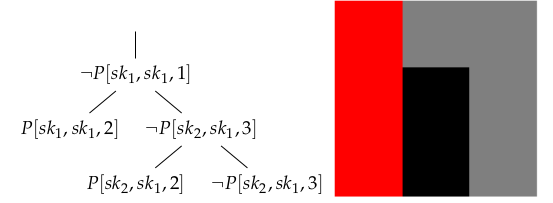
\includegraphics[width=8cm]{ART_Lampert/fig1.png}
\end{center}
\caption{Regularity in the narrow sense in ATP for (\ref{repclause})}
    \label{rep}
\end{figure}

Examples suggest that regularity in the narrow sense can be generalized to cases in which the proof search runs in endless loops without repeating expressions in the narrow sense. As Figure \ref{quine} illustrates for the simple clause (\ref{boergerS33clause}) with only infinite models, the proof search may encounter an obvious nesting scenario. We can identify a law that governs how the sequence of formulas develops from the sequence alone, without considering the clauses or instructions of the proof search algorithm. In this case, the sequence of inference steps is, in fact, governed by a repeating pattern, albeit without strict repetition of the same expression. The question is whether we can infer from the finite repetition of a pattern that it will repeat endlessly. We will explain by counter-examples why this question has a negative answer.

\begin{figure}[ht]
\begin{center}
%\begin{forest}
%[{}
%[{$\neg P[x_{1_1},sk_1(x_{1_1}), 1]$}
%[{$P[x_{1_1}, sk_1(x_{1_1}), 2]$}]
%[{$\neg P[x_{1_1}, sk_1(sk_1(x_{1_1})), 3]$}
%[{$P[x_{1_1}, sk_1(sk_1(x_{1_1})), 2]$}]
%[{$\neg P[x_{1_1}, sk_1(sk_1(sk_1(x_{1_1}))), 3]$}
%[{$P[x_{1_1}, sk_1(sk_1(sk_1(x_{1_1}))), 2]$}]
%[{$\neg P[x_{1_1}, sk_1(sk_1(sk_1(sk_1(x_{1_1})))), 3]$}
%]]]]]
%\end{forest}
%\vspace{0.25cm}
%\includegraphics[width=6cm]{quine.png}
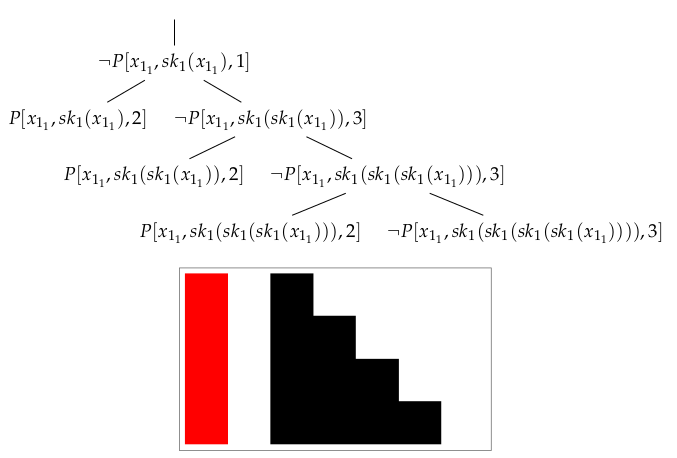
\includegraphics[width=8cm]{ART_Lampert/fig2.png}
\end{center}
\caption{Regularity in the broad sense in ATP for (\ref{boergerS33clause})}
    \label{quine}
\end{figure}


There are, of course, more complicated cases of looping than the one shown in Figure \ref{quine}, and the proof search may become too messy for a human to identify any pattern at all. However, this may be a problem that one may hope to overcome by means of translation into other, more perspicuous notations, or it may be a problem of human pattern identification capabilities that one may hope to overcome by means of machine learning. Thus, one may strive for intricate pattern detection for endless loops in ATP.
Our question is how to explain why this endeavor is hopeless.
Our philosophical motivation for this question is to explain why a diagrammatic (or ``iconic'')
conception of logic that claims that logical properties, such as provability, are reducible to pattern detection in a suitable notation fails when applied to the whole realm of FOL \parencite[cf.][for details about this diagrammatic (or iconic) conception of logic, which is based on insights from Wittgenstein's early work]{Lampert3}. We maintain that this conception works only for normal form transformations of \emph{fragments} of FOL (see p. \pageref{normalforms} above); we intend to show that and explain by counter-examples why the reducibility claim is incorrect when applied to a general proof search in FOL.


We designate a purported general decision criterion referring to a \emph{finite part} of a computable sequence, wherein this finite part repeats a pattern, as a ``loop criterion''. This criterion is employed to justify an inference from finite repetitions to endless repetitions and, thus, to determine unprovability. It generalizes the regularity criterion. We aim to answer the following question by providing concrete examples: Why is it impossible to generalize the regularity criterion to correctly determine unprovability by means of a general loop criterion in a complete and automated proof search?

To our knowledge, this question has not been raised in the literature thus far. We shall address this question by considering a simple undecidable class of FOL formulas, namely, the ones which can be expressed as a set of Krom--Horn clauses%, and their translation into pure FOL formulas
. Krom--Horn clauses are clauses with at most two members, with at most one being non-negated. Specifically, we will consider only sets of Krom--Horn clauses derived from translations of so-called splitting Turing machines (STMs). We specify STMs for the purpose of making evident the limitations of a decision criterion specified in terms of a loop criterion. By translating STMs into a special sort of Krom--Horn clauses, we can demonstrate how the halting problem for STMs transforms into the decision problem for the corresponding Krom--Horn clauses. Although the deterministic proof search for Krom--Horn clauses % and of their corresponding pure FOL translations 
will mirror the behavior of STMs, our approach does not involve \emph{expressing}
STMs in FOL (as is usually done in undecidability proofs), nor do we employ diagonalization or any axioms (theory) in addition to the pure translation of the input and instructions of STMs.
Instead, we mimic the execution of deterministic STMs via a deterministic proof search to show the impossibility of specifying a general criterion for detecting endless loops within an exhaustive proof search in FOL. Our discussion will not only dispense with the diagonal method in combination with hypothetical (counterfactual) reasoning, but will also abstain from \emph{expressing} Turing machines by means of FOL formulas in relation to their intended interpretation. Rather, it will be purely syntactic and, thus, demonstrable through our implementation of the translation and proof search procedures. In fact, the translations of STMs to Krom-Horn clauses will merely serve as a heuristic to generate Krom-Horn clauses with certain logical properties which can also be proven independent of their relation to STMs.

%%%%%%%%%%%%%%%%%%%%%%%%%%%%%%%%%%%%%%%%%%

\section{From the halting problem to the \textit{Ent\-schei\-dungs\-problem}}\label{results}

We begin by introducing STMs and explain why an endeavor to solve the halting problem for STMs based on patterns in their evolution is futile (section \ref{STMsec}). As the main content of our paper, we
then show how this explanation transfers to the \emph{Entscheidungsproblem} by considering a proof search for clauses with skolemization (section \ref{tableauxsec})% and for pure FOL formulas without Skolemization (section \ref{NNFsec})
.


\subsection{Splitting Turing Machines}\label{STMsec}

An STM, or splitting Turing machine, is an automaton equipped with a circular tape consisting of cells that can be split. The specifications and behavior of STMs are defined as follows:

\begin{description}
\item[Def. (\textbf{Splitting Turing Machine, STM}):] An \label{DefSTM} STM is described by a tuple $S =$ $(Q, \Sigma, f, q_1,$ $q_f, c_n)$, where $Q$ and $\Sigma$ are the finite sets of states and tape symbols, respectively; $q_1\in Q$ is the initial state; $q_f \in Q$ is the halting state; $c_n$ is the initial tape of size $n$ that defines the symbols for all $n$ initial positions of the machine; and the transition function $f$
is defined for all $q\in Q$, except $q_f$, and for all read symbols $\sigma$\footnote{For simplicity, the definition may omit specifying the value of $f$ for pairs of states and symbols that are never reached.}.
\end{description}

We write $f$ as a list of transition rules. Each rule is expressed as a quadruple $t = (q_x, \sigma, v, q_y)$, with initial state $q_x$, read symbol $\sigma$, instruction $v$, and next state $q_y$. The possible instructions are as follows:

\begin{description}
\item[W$s$:] write the symbol $s$, $s \in \Sigma$;
\item[S:] split the current cell, duplicating its content on the right (clockwise) of the current cell;
\item[L:] move the scanner counterclockwise;
\item[R:] move the scanner clockwise.
\end{description}

STMs are universal machines because they can simulate clockwise Turing machines (CTMs), which are universal; \parencite[cf.][pp.107-109]{Neary}.\footnote{Demonstrating that CTMs can be simulated by STMs is straightforward. Essentially, CTMs are automata that move to the right after every instruction and either write one symbol on the tape or split one cell of the tape and write two symbols in the split cells. These operations are all available in STMs.} Therefore, if the halting problem is solvable for STMs, then it is solvable for all Turing machines.

It is a well-known fact that even Turing machines of minimal complexity can generate rather irregular sequences in their evolution; cf., e.g., Figure \ref{messy} for the 5-state, 3-symbol STM described by (\ref{STM0}) (the color diagram evolves from left to right, cf. p. \pageref{colordia} for the explanation of color diagrams for Turing machines).

\begin{table}[!ht]
\begin{eqnarray}
\hspace{-0.5cm}& \begin{tabular}{ll}
$Q$: & $\{P,Q1,Q2,Q3,H\}, q_{1}:P, q_{f}:H$,\\
$\Sigma$: & $\{0,1,2\}$,\\
$f$: & \hspace{-0.2cm}\begin{small}\begin{tabular}{l}$\{\{P,1,\{L\}, P\},\{P,0,\{W,1\},Q1\},\{P,2,\{R\},Q3\},\{Q1,1,\{R\},Q2\},$\\
$\{Q1,0,\{R\},Q2\},\{Q2,1,\{W,0\},Q1\},\{Q2,2,\{L\},P\},\{Q3,1,\{S\},Q1\}\}$,\end{tabular}\end{small}\\
$c_{2}$: & $\{1, 2\}$.
\end{tabular} & \label{STM0}
\end{eqnarray}
\caption{A 5-state, 3-symbol STM inducing the irregular color diagram in Fig. \ref{messy}}
\end{table}

\begin{figure}[!ht]
    \centering
    
\includegraphics[width=12.5cm]{ART_Lampert/messy.png}
\caption{Color diagram of the evolution of the STM (\ref{STM0}) over 150 steps}
    \label{messy}
\end{figure}

One might wonder whether seemingly irregular sequences already indicate that a decision procedure based on pattern detection for identifying endless looping is futile. However, regularity depends on notation.
A different notation may well enhance the possibility of solving decision problems\footnote{Cf. \parencite{Lampert2} for a general discussion of this claim.}, e.g., by converting irregular sequences into regular ones.
Approximating a number by means of different sequences in different notations, which can be translated into each other, is one example of this; cf. Table \ref{regular}. Take the example of square roots: while their representations in decimal notation might not exhibit a discernible pattern, their regular continued fractions demonstrate \emph{periodicity}, allowing for easier identification.
Similarly, one could argue that by translating the irregular sequence generated by an STM into a regular one through notation transformation, a recognizable pattern might emerge. Our approach of translating STMs into clauses or FOL formulas, and subsequently generating sequences of inference steps by applying a logical calculus, allows us to explore the relations between sequences in different notations with respect to the resulting patterns.
The normal form transformations employed to solve decision problems for fragments of FOL, as discussed earlier (cf. p. \pageref{normalforms}), illustrate how the ability to solve decision problems in logic depends on a notation that may reveal logical properties in the form of common patterns. From the practical standpoint of a software engineer, one might also wonder whether machine learning could outperform humans and gain the ability to decide problems (at least to a reliable degree) by learning from patterns in a training database.

However, it can be demonstrated through a representative example that attempting to solve the halting problem based on patterns of STM sequences or to solve the \emph{Entscheidungsproblem} based on patterns of sequences of inference steps is futile, irrespective of the extent to which irregular sequences can be transformed into regular ones.
We can demonstrate this by considering \emph{regular} instead of irregular sequences, i.e., by considering cases in which a pattern is \textit{indeed} found. We first do this for sequences computed by STMs and the question of solving the halting problem and then ask whether the same approach can be extended to sequences in ATP and the \emph{Entscheidungsproblem}. Thus, we do not explain undecidability due to the lack of detectable patterns in unsuitable notations. Instead, we explain undecidability due to the impossibility of distinguishing properties such as halting / non-halting in the case of STMs and refutability / satisfiability in the case of FOL \emph{despite of the identification of patterns}. 

Our example, in which STM1 and STM2 are specified as shown in Table \ref{STM1} and their color evolution diagrams are presented in Figure \ref{STM12}, demonstrates that mere repetition of a regular pattern is not sufficient to decide that a Turing machine is nonhalting. STM2 differs from STM1 solely by the replacement of one of the halting instructions with a nonhalting instruction. Their evolution diagrams remains identical for the initial 78 steps, encompassing a complete repetition of a regular pattern. However, 
STM1 halts in the next step, while STM2 continues forever in a regular manner.

\begin{table}
\begin{eqnarray}
\hspace{-0.5cm}& \begin{tabular}{ll}
$Q$: & $\{P,P1,P2,P3,P4,H\}, q_{i}: P, q_{f}: H$,\\
$\Sigma$: & $\{1,2,3,4\}$,\\
$f$: & \hspace{-0.2cm}\begin{small}\begin{tabular}{l}$\{\{P,1,\{W,2\}, P1\},\{P,2,\{R\},P\},\{P,3,\{R\},P4\},$\\
${\bf \mbox{\bf STM1:} \{P,4,\{W,4\},H\}, \mbox{\bf STM2:} \{P,4,\{W,4\},P1\}}$,\\
$\{P1,1,\{R\},P1\},\{P1,2,\{R\},P1\},\{P2,3,\{R\},P\},\{P1,4,\{R\},P\},$\\
$\{P2,1,\{R\},P2\},\{P2,2,\{W,1\},H\},\{P2,3,\{R\},H\},\{P2,4,\{R\},P3\}$,\\
$\{P3,1,\{S\},P\}, \{P3,2,\{S\},H\}, \{P3,3,\{R\},H\},\{P3,4,\{W,1\},H\},$\\
$\{P4,1,\{R\},P4\},\{P4,2,\{W,1\},P4\}, \{P4,3\{R\},P2\}, \{P4,4,\{R\},P4\}\},$
\end{tabular}\end{small}\\
$c_{5}$: & $\{1,3,1,1,4\}$.
\end{tabular} & \nonumber 
\end{eqnarray}
\caption{STM1 (halting) and STM2 (not halting), differing by one instruction  \label{STM1}}
\end{table}

\begin{figure}
    \centering
    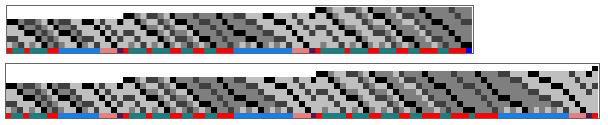
\includegraphics[width=12.5cm]{ART_Lampert/STM12.png}
\caption{Color diagrams for STM1 and STM2 up to 100 steps}
    \label{STM12}
\end{figure}

It is easy to describe the difference of the functions that the instructions of STM1 and STM2 implement. Both take as input two sequences of 1s, $a$ and $b$, separated by the symbols 3 and 4. While $a$ increments by 1 in each iteration, $b$ remains constant. STM1 halts when $a > b$, whereas STM2 goes on with incrementing $a$ forever. Yet, describing the implemented functions does not amount to provide a general decision criterion for distinguishing finite from infinite loop processes. Recall that, from the point of view of metalogic, it is possible to mechanically decide for any members of an arbitrary \emph{finite} set of STMs (that may well include STM1 and STM2) whether they halt or do not halt, cf. p. \pageref{metafinite}. It is even possible to devise an algorithm that decides, for an infinite set of STMs that includes STM1 and STM2, whether its members halt or do not halt. This can be done by considering special forms of machines, e.g., machines that implement Do-until loops that do not modify the loop counter during the loop, but only increment or decrement the counter after each loop until a certain value is reached and, additionally, each single loop is known to end after a finite number of steps. Yet, what is in question is a decision criterion that applies to \emph{all} STMs, thereby distinguishing finite from infinite loop processes \emph{in general}, solely based on detecting repeating patterns, regardless of an upper bound on loop iterations. This becomes imperative when dealing with STMs featuring While-loops where termination hinges not on reaching a predefined counter but on satisfying a specific condition. Our pair of machines, STM1 and STM2, epitomizes the fundamental challenge of formulating a \emph{general} criterion for escaping a loop by pattern detection. Unlike the counterfactual diagonal case, such a pair comprises concrete STMs, which enables the translation of the problem to a factual pair of expressions within FOL and its illustration by real automated proof search.

In investigating sequences, we assume that it is possible to identify mechanically loops that repeat a certain pattern. In the case of STM1 and STM2, e.g., the looping process starts from configurations differing solely in the increasing number of 1s in the first sequence $a$ of 1s. Within each iteration of the loop, the same instructions are applied in the same order, with only the number of applications of these instructions varying in each repetition due to the increasing nesting. A universal machine can identify the looping process by detecting the successive increase of nesting and the repeating succession of rule applications resulting from it. Given these assumptions, the question arises whether it is possible to infer non-halting behavior from the identification of a looping process. 

Pairs of STMs such as STM1 and STM2 show that and explain why the answer to this question is negative. 
These machines share a looping process; yet, while STM1 escapes the loop and halts, STM2 repeats the looping process endlessly. All of the halting instructions in both STM1 and STM2, except the one absent in STM2, are irrelevant as their conditions will never be met. STM2 does the same as STM1 with the only difference being that it continues its execution after each comparison of the increasing number $a$ with $b$.  A loop criterion is refuted by the fact that, by simply redefining a relevant instruction where a halting condition will be satisfied, one can specify a machine that behaves likewise but continues its execution while the original halts. Clearly, examples such as STM1 and STM2 can be extended to an arbitrary number of
pairs of halting and nonhalting machines by redefining relevant halting instructions.

Our refutation implies that STM2 can no longer be decided as nonhalting according to a pure loop criterion that is based on nothing but \label{assumption} the detection of a pattern within a \emph{finite} part of a computable sequence. Note that, by increasing the second number $b$ against which the first number $a$ is compared, we can arbitrarily increase the number of repetitions executed before STM1 comes to a halt. Therefore, a loop criterion cannot be rescued by \emph{merely} increasing the number of repetitions under consideration.

We do not refute a loop criterion by objecting that it may be challenging to identify patterns in a suitable notation. Instead, our refutation stems from the fact that such a criterion fails to provide a sufficient condition for nonhalting when loops can be mechanically identified. In what follows, our aim is to extend this straightforward refutation of the validity of a loop criterion for solving the halting problem to the attempt of applying such a criterion to solve the \emph{Entscheidungsproblem} within ATP. In this context, it is not equally straightforward to see the failure
of a loop criterion when employed as a general decision criterion.
Since regularity and decidability depend on notation, refuting a loop criterion for sequences generated by STMs does not \emph{immediately} imply refuting it for ATP. To establish this,
we must demonstrate how the (trivial) impossibility of solving the halting problem based on a loop criterion can be transposed to show the (nontrivial) impossibility of solving the \emph{Entscheidungsproblem} based on a loop criterion.


Furthermore, proofs are typically examined in logic without considering their relation to the execution of Turing machines. One may even harbor reservations concerning the endeavor to overload FOL formulas with interpretations that go beyond a pure proof-theoretic point of view. Consequently, one may be inclined to abstain from \emph{expressing} Turing machines by means of FOL formulas by making use of interpretations $\Im$ of FOL-expressions intending to capture the states, the tape and the instructions of TMs.\footnote{Cf. \parencite{Lampert2}, section 5, which criticizes semantic versions of undecidability proofs of FOL. Our purely syntactic version of mimicking the behavior of STMs circumvents these concerns entirely.} To circumvent these reservations, we will show in the following that and how the impossibility of specifying a loop criterion for the halting problem can be extended to the impossibility of doing this within ATP without \emph{expressing} STMs within the language of FOL. Instead, we will show how to mimic the behavior of STMs in a deterministic proof search for the rather simple case of Krom--Horn clauses. % and their translations into pure FOL.

\subsection{ATP-search}\label{tableauxsec}

We proceed to show how our explanation of the invalidity of a loop criterion as a decision criterion for the halting problem can be extended to establish the unsolvability of the decision problem for FOL by employing a loop criterion. For this sake, we specify an ATP-search that emulates the behaviour of STMs. This can be accomplished by utilizing the well-known ATP-search within a tight connection tableau calculus, which is identical to an ATP-search in the also well-known linear resolution calculus for the special case of Krom-Horn clauses that we consider, cf. footnote \ref{resolu}. The crucial point is that the ATP-search, in fact, produces repeating patterns in terms of regularity not only in the narrow but also in the broad sense. Thus, we demonstrate that increasing complexity through the endless iterative application of inference rules, which is a necessary feature of any complete calculus for FOL, cannot be circumvented by a loop criterion, even in the case where the ATP-search generates discernible repeating patterns that would enable the application of such a criterion. Note that mimicking the behaviour of TMs by ATP-search is not a trivial task: Our translation of STMs into Krom-Horn clauses is tailored to specifically emulate the behaviour of a certain type of TMs by a particular ATP-search. Different types of TMs (e.g., those without splitting cells), other notations of FOL-expressions (e.g., without skolemization) and other correct and complete calculi (e.g., those requiring iterative application of $\wedge$I) may well render the application of a loop criterion impractical, if not impossible. In these cases, decidability through pattern detection is thwarted due to the absence of discernible or repeated patterns. However, this is a feature of notation that one can hope to overcome by the reduction to proper notations and calculi. We show that even in the case of such a reduction, a loop criterion remains unreliable.

Let us first enumerate the elements we will use for representing the machine and the contents of its tape:

\begin{enumerate}
\item A Skolem constant $sk_G$.
\item A Skolem constant $sk_s$ for every $s \in Q$. \label{sks}
\item A unary Skolem function $sk_a$ for every $a \in \Sigma$. 
\item A predicate letter $P_s$ with arity $n+1$ for an STM with $n$ initials cells for every $s \in Q$.
\item Some auxiliary predicate letters, to be defined below.
\end{enumerate}

An STM in a certain state and with certain symbols written on its tape will be represented by a literal (i.e. an atomic formula or its negation) as follows: the different states of the machine will be represented by different predicate letters (and, additionally, by different Skolem constants, see \ref{sks} above; this redundancy is introduced merely for simplicity); the tape of the machine will be represented by the arguments of the predicates, with the first argument representing the position of the scanner of the machine; the different symbols that may be written on the tape of the machine will be represented by different Skolem functions; finally, the potentially infinite nature of the tape (due to the splitting operation) will be represented by the potentially infinite nesting of these Skolem functions. The Skolem constant $sk_G$ marks the end (the ``ground'') of nesting.

From here on, we will employ the metavariable $\alpha$ to represent variables that run through the values of $\Sigma$ and the metavariable $\beta$ to represent variables that run through the values of $Q$. Additionally, we stipulate that the first argument of the predicates will always represent only a \textit{single} cell in the machine. The reason for this stipulation is merely practical.

We assume that the tape is initially filled with $s_1, s_2,\cdots, s_n$, where all $s_i\in\Sigma$. 
Given that we utilize the tight connection calculus beginning with a single negated literal, cf. p. \pageref{onenegative}, our initial clause contains only one negated literal and our clauses of length 2 will start with a positive and end with a negated literal.
The initial clauses of the FOL formula in clause normal form are as follows:

\begin{equation}
\{\neg F_{aux0}[sk_G, ..., sk_G]\} \label{ini1}
\end{equation}

\begin{equation}
\{F_{aux0}[x_1, \ldots, x_1], \neg P_{q_1}[sk_{s_1}(x_1), sk_{s_2}(x_1), \ldots, sk_{s_n}(x_1), sk_G]\} \label{ini2}
\end{equation}

The arity of $F_{aux0}$ is $n$, i.e. the number of initial cells.
Note that the tape, which is of size $n$, is represented by $n+1$ arguments in predicate letters $P_s$ such as $P_{q_1}$.
The ($n+1$)-th argument will always be $sk_G$, which is useful for the specification of Rule R below.

The ATP-search starts by deriving $\neg P_{q_1}[sk_{s_1}(sk_G),sk_{s_2}(sk_G), \ldots,$ $sk_{s_n}(sk_G), sk_G]$ from (\ref{ini1}) and~(\ref{ini2}). We could have simplified (\ref{ini1}) and (\ref{ini2}) to this literal. However, we want our clauses to be easily translatable into pure FOL-expression without skolemization, cf. section \ref{materials}. For this sake, skolem functions should not occur within skolem-functions prior to substitutions in the initial clauses, i.e. prior to substitution of variables during the application of inference rules. For the same reason,  we impose the general restriction that, in the clauses, the only permissible argument for the Skolem functions $sk_a$ for every $a \in \Sigma$ is $x_1$. \label{x1rest}

For the halting state $q_f$, we add the following unit clause:

\begin{equation}
\{P_{q_f}[x_1, ..., x_n, sk_G]\}
\end{equation}

Let us now see which clauses are needed for every kind of transition rule. We assume that the description of each rule is given in the format $(q_x, \sigma_1, v, q_y)$.

We will omit the translation of Rule L since it is analogous to Rule R and since we do not need it in our examples or for our argument. Rules W and S are straightforward and obviously yield a literal representing the resulting state and tape of the corresponding STM.

\subsubsection{Rule W}

Suppose that the symbol to be written is $\sigma_2$. To represent Rule W, we simply add the following clause:

\begin{equation}
 \{P_{q_x}[sk_{\sigma_1}(x_1), x_2, x_3, \ldots, x_{n+1}],
 \neg P_{q_y}[sk_{\sigma_2}(x_1), x_2, x_3, \ldots, x_{n+1}]\}
\end{equation}

\subsubsection{Rule S}

To represent Rule S, we add the following clause:

\begin{small}
\begin{equation}
\hspace{-0.95cm} \{P_{q_x}[sk_{\sigma_1}(x_1), x_2, x_3, \ldots, x_{n+1}],
 \neg F_{auxS_{\sigma_1}}[sk_{\sigma_1}(x_1), x_2, x_3, \ldots, x_{n+1}, sk_{q_y}]\}
\end{equation}
\end{small}

Additionally, we include the following clauses in the set of clauses (these clauses are included only once, not for every Rule S dictating the machine's behavior):

\begin{equation}
 \{F_{auxS_{\alpha}}[x_2, x_1, x_3, \ldots, x_{n+1}, sk_\beta], \neg P_\beta[x_2, sk_\alpha(x_1), x_3, \ldots, x_{n+1}]\}
\end{equation}

The rationale for the introduction of the auxiliary predicate letters $F_{auxS_{\alpha}}$ is that they allow for the representation of the splitting of the cells while obeying the restriction that, in the clauses, the only permissible argument for the Skolem functions $sk_a$ for every $a \in \Sigma$ is $x_1$, cf. p. \pageref{x1rest}.

\subsubsection{Rule R}

The specification of Rule R is considerably more intricate compared to Rules W and S. Let us begin with an example to illustrate how mimicking this rule in a tight connection tableau calculus unfolds. Imagine that at a given instant during the machine's execution, its state $q_x$ and the tape $[1,2,3,4,5,6]$ are represented by the following literal, which appears on a leaf of a certain open branch of the tableau:\\

$P_{q_x}[sk_1(sk_G), sk_2(sk_3(sk_4(sk_G))), sk_5(sk_6(sk_G)), sk_G]$\\

The idea is that at the end of the mimicking operations in the tableau, we shall obtain the following literal on the leaf of this branch:\\

$P_{q_y}[sk_2(sk_G), sk_3(sk_4(sk_5(sk_6(sk_G)))), sk_1(sk_G), sk_G]$\\

\noindent representing the tape $[2,3,4,5,6,1]$ and the machine in state $q_y$. This evolution during the application of the rules of the tableau calculus is designed to mimic the fact that the header of the machine moves one position to the right on the tape, transitioning from the state $q_x$ to the state $q_y$.

To ensure that Rule R will be applied only if the scanned symbol is $\sigma_1$, we include the following clause:

\begin{equation}
\hspace{-0.5cm} \{P_{q_x}[sk_{\sigma_1}(x_1), x_2, x_3, ..., x_{n+1}\},
 \neg F_{aux_R}[sk_{\sigma_1}(x_1), x_2, x_3, ..., x_{n+1},sk_{q_y}]\} \label{FauxR}
\end{equation}

Now, we start moving the symbols to the right. Initially, we add the following clauses to the set of clauses:

\begin{equation}
\begin{tabular}{c}$\{F_{aux_R}[x_2, sk_\alpha(x_1), x_3, \dots , x_{n+2}],$ \\
$\neg F_{aux1_\alpha}[sk_\alpha(x_1), x_1, sk_G, x_3, \ldots, x_{n}, x_2, x_{n+1},x_{n+2}]\}$\end{tabular} \label{Faux1}
\end{equation}

The rationale for the arguments of $F_{aux1_\alpha}$ will only be made clear after the following operations 1 to 4 are explained. We need to perform the following operations with the arguments of $F_{aux1_\alpha}$ to represent the tape after the execution of the rule:

\begin{enumerate}
\item Set the first argument to $sk_\alpha(sk_G)$ (for the particular value of $\alpha$ in question).
\item Pop the represented symbols on the tape contained in $x_1$ (second position of $F_{aux1_\alpha}$), push them over the third position, and finally remove the second position.
\item Pop the inverted $x_1$ obtained in operation 2 above and push these symbols over $x_3$ to put them in the right order, again removing the second position.
\item Use the last argument of $F_{aux1_\alpha}$, which stores the next state, to finally construct the correct predicate letter.
\end{enumerate}

Regarding clauses (\ref{Faux1})--(\ref{Pbeta}), and unlike clause (\ref{FauxR}) above, we anticipate that these clauses do not need to be added for \textit{every} Rule R. Instead, we include them only once.

To accomplish the first task, we include the following clauses:

\begin{small}
\begin{equation}
  \hspace{-1cm}  \{F_{aux1_\alpha}[x_2, x_3, \ldots, x_{n+3}, x_1, x_{n+4}], \neg F_{aux2}[sk_\alpha(x_1), x_3, \ldots, x_{n+3}, x_1, x_{n+4}]\}\label{Faux2}
\end{equation}
\end{small}

To accomplish the second task, we include the following clauses:

\begin{equation}
\{F_{aux2}[x_2, sk_{\alpha}(x_1), x_3, \ldots, x_{n+4}], 
\neg F_{aux3_{\alpha}}[x_2, x_1, x_3, \ldots, x_{n+4}]\}
\end{equation}

\begin{equation}
\hspace{-0.5cm} \{F_{aux3_{\alpha}}[x_2, x_3, x_1, x_4, \ldots, x_{n+4}],
\neg F_{aux2}[x_2, x_3, sk_{\alpha}(x_1), x_4, \ldots , x_{n+4}]\}
\end{equation}

\begin{equation}
\{F_{aux2}[x_1, sk_G, x_2\ldots, x_{n+3}],
\neg F_{aux4}[x_1, x_2 \ldots, x_{n+3}]]\}
\end{equation}

The third task is similarly completed by including the following clauses:

\begin{equation}\{F_{aux4}[x_2, sk_{\alpha}(x_1), x_3, \ldots, x_{n+3}], 
\neg F_{aux5_{\alpha}}[x_2, x_1, x_3, \ldots, x_{n+3}]\}
\end{equation}

\begin{equation}
\{F_{aux5_{\alpha}}[x_2, x_3, x_1, \ldots, x_{n+3}],
\neg F_{aux4}[x_2, x_3, sk_{\alpha}(x_1), \ldots, x_{n+3}]\}
\end{equation}

\begin{equation}
\{F_{aux4}[x_1, sk_G, x_2 \ldots, x_{n+2}],
\neg F_{aux6}[x_1, x_2 \ldots, x_{n+2}]\}
\end{equation}

Finally, to accomplish the fourth task, we include the following clauses:

\begin{equation}
\{F_{aux6}[x_1, \ldots, x_{n+1}, sk_\beta],
\neg P_\beta[x_1, \ldots, x_{n+1}]\} \label{Pbeta}
\end{equation}

\subsubsection{Mimicking the evolution of STMs}

Applying the rules of our translation procedure to a given STM yields a set of Krom--Horn clauses. The initial and final states are translated into clauses of length 1, while all instructions are translated into clauses of length 2 with exactly one non-negated literal. Our presumed complete ATP procedure based on tight connection tableau, initiated with clauses containing only negated literals, makes it possible to mimic the execution of deterministic STMs via a very simple deterministic ATP process. It starts with the initial clause, since this is the only clause that contains only negated literals. Subsequently, there is precisely one expansion step to be iteratively executed (this fact readily follows from inspection of the provided set of clauses).
Reduction steps, which do occur in a complete tableau proof search for the whole realm of FOL, are absent in the complete tableau proof search for the special case of Krom-Horn clauses.
The proof search terminates if and only if the halting state is reached. Since the proof procedure is deterministic, any proof is necessarily of minimal length. Incidentally, the same is true for a proof search within the linear resolution calculus, which does not differ significantly from the proof search in tableaux in the special case of Krom--Horn clauses.\footnote{Full resolution reduces to binary resolution, factorization is not needed, the expansion rule and binary resolution are identical in this case, and \parencite{Henschen} have shown that linear \emph{input} \label{resolu} resolution is complete for Horn clauses.}

Although ATP mimics the evolution of STMs, there is no one-to-one correspondence but rather a one-to-many correspondence between the steps of the STMs and the steps in our tableau calculus. The primary reason for this is Rule R, which entails a pop--push process for the Skolem functions in positions two and three of the predicates to achieve the correct order of the arguments in the Skolem functions.
However, one can compare the literals in the ATP process following each translation of an instruction with the tape after the performance of an instruction during STM execution. This can be seen, for example, by contrasting the color diagrams of the STM sequences with those of the ATP process; see, e.g.,
Figure \ref{STM12} and Figure \ref{STM12skolem} (cf. p. \pageref{colordia} for the explanation of color diagrams).

\begin{figure}
    \centering
    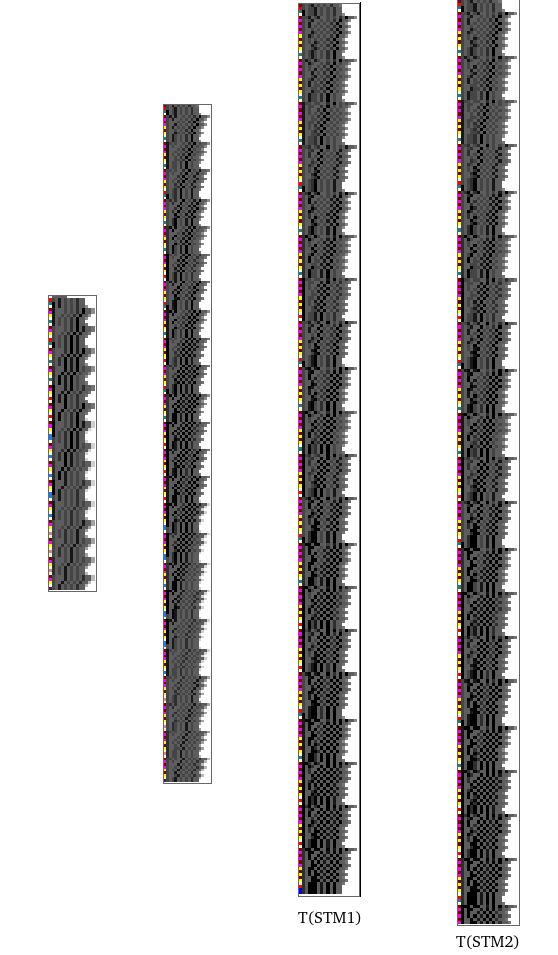
\includegraphics[width=10.5cm]{ART_Lampert/STM12tableauxtotal.png}
\caption{Color diagrams of the proof searches for T(STM1) and T(STM2),
showing that although both are governed by the same pattern before the proof search for T(STM1) terminates, only the proof search for T(STM2) continues to repeat this pattern.}
    \label{STM12skolem}
\end{figure}

The translation T(STM1) of STM1, which is a provable formula, differs by only one literal in one clause from the translation T(STM2) of STM2, which is a satisfiable formula. The automated proof of T(STM1) in tableaux takes 634 steps. Figure \ref{STM12skolem} shows the evolution diagrams for T(STM1) and T(STM2), divided into three parts (the partial diagrams are meant to be read from top to bottom). The outermost left partial diagram covers steps 1--96, while the subsequent partial diagram encompasses steps 97--346 after the first splitting. The third partial diagram shows steps 347--634 for T(STM1) after the second splitting, while the last partial diagram depicts steps 347--640 for T(STM2) after the second splitting. The third and fourth partial diagrams diverge only at step 634, which is the last step in the proof of T(STM1), while the proof search for T(STM2) continues indefinitely. The patterns repeat after each splitting, becoming more nested; this extends the pop--push processes without causing new symbols to be written or new states to be entered relative to the previous sequence of inference steps within one splitting period. Thus, similar to the computable sequences of STM1 and STM2, the sequences of inference steps for T(STM1) and T(STM2) share the same repeating pattern. However, this pattern endlessly repeats only in the proof search for T(STM2). This demonstrates that the invalidity of the loop criterion for deciding whether halting occurs in the case of STM1 and STM2 extends to the invalidity of deciding provability for T(STM1) and T(STM2) based on a loop criterion for an automated proof search within a tableau or resolution calculus.\footnote{T(STM1) and T(STM2) each contain 79 clauses and thus are too long to be printed here. All automatically generated diagrams and translations from STM1 and STM2 can be viewed at %{ANONYMIZED}{here}. 
\href{https://github.com/TimmLampert/KromHornSolver}{\nolinkurl{www.github.com/TimmLampert/KromHornSolver}}.%{here}.
\label{linkfoot} 
The printed output of the color diagrams and their symbolic expressions is 
\href{http://www2.cms.hu-berlin.de/newlogic/webMathematica/Logic/STM1.pdf}{125}
and 
\href{http://www2.cms.hu-berlin.de/newlogic/webMathematica/Logic/STM2.pdf}{133}
pages long.}

Since we can produce an arbitrary number of further pairs of STMs for this case, we can also generate an arbitrary number of further pairs of provable and satisfiable formulas that share a regular sequence of inference steps up to an arbitrary length. This demonstrates the futility of specifying a loop criterion for ATP-search.

\section{KromHornSolver}\label{materials}

In contrast to metamathematical proof methods, such as the diagonal method, we base our results on examples and computation. STMs and their automated translations into Krom--Horn clauses are especially suited for explaining undecidability in terms of pattern detection in ATP. To aid the visualization of our argument, we compute color diagrams instead of printing complex symbolic expressions and proofs.

Our results are based on a \emph{Mathematica} program called \emph{KromHornSolver}, which we implemented ourselves.\footnote{This program is available at \href{https://github.com/TimmLampert/KromHornSolver}{www.github.com/TimmLampert/KromHornSolver}, %{here},
and an implementation of it can be accessed at \href{https://www2.cms.hu-berlin.de/newlogic/webMathematica/Logic/kromhornsolver.jsp}{www2.cms.hu-berlin.de/newlogic/webMathematica/Logic/kromhornsolver.jsp}.}%{here}.}
This program not only conducts proof searches for clauses but also for corresponding FOL-formulas without skolemization, which are generated from the clauses. The ATP-proof search for those FOL-formulas is based on a different calculus that applies the rule $\wedge$I instead of the expansion rule prior to universal quantifier eliminations. Avoiding skolemization makes it impossible to reproduce the repeating patterns of the evolution of STMs in the case of splitting cells, thereby precluding the application of a loop criterion. This occurs due to the fact that the splitting tape can no longer be represented by $P$-literals with increasing nested skolem-functions but only by several $P$-literals dispersed among other literals in different scopes of different quantifiers, which increase in number by the splitting process. Consequently, there is no remaining main branch of an ATP-search with $P$-literals corresponding to the evolution of the STM. Instead, the evolution of STMs is encoded in a complex FOL-expression with literals not arranged in a regular sequence but distributed across different scopes of different quantifiers. By implementing two different ATP-searchs based on two different notation (with and without skolemization), we intended to underscore the impact of notation and calculus on pattern detection. 

The \emph{KromHornSolver} takes an STM plus an upper bound for execution as its input. It then performs the following steps:
\begin{description}
\item[Step 1:] The array for the steps of the STM is generated its color diagram is printed.
\item[Step 2:] The STM is translated into clauses with Skolem functions and into a pure FOL formula (without Skolem functions).
\item[Step 3:] The deterministic tableau is generated for the clauses and its color diagram is printed.
\item[Step 4:] The tableau proof is translated into a pure FOL formula encoding the corresponding proof in proof search without skolemization and its color diagram is printed.
\item[Step 5:] Attempts to specify a loop criterion are checked.
\end{description}

Step 5 refuted the correctness of a loop criterion for the ATP-search for clauses with skolemization, while the corresponding ATP-search for pure FOL-formulas without skolemization does not allow for specifying a general loop criterion due to the lack of regular sequences. In both cases, it becomes impossible to decide satisfiability by identifying repeating patterns.

\section{Conclusion}\label{discussion}

Our main concern is to \emph{demonstrate that} and to \emph{explain why the particular putative attempt} to solve the \emph{Entscheidungsproblem} within \emph{given} calculi and proof search algorithms by adding a general loop criterion is futile, rather than \emph{proving in general that} the \emph{Entscheidungsproblem} is unsolvable \emph{by any method}. Our explanation is based on mimicking STM sequences in ATP. However, this does not mean that our explanation hinges on the translation of STMs into FOL. We merely use this translation method as a heuristic to generate pairs of sequences in ATP that share a repeating pattern. Once these sequences are generated, the validity of a loop criterion for an ATP-search yielding repeating patterns is directly refuted by the fact that an infinite sequence for an unprovable formula and a finite sequence for a provable formula contain the same repeating pattern.

Our discussion of the limits of a loop criterion can be seen as an instance of the general insight that finite, regular parts of computable sequences lack an unambiguous continuation. However, we argue that simply referring to this insight in a general context is insufficient when discussing ATP. Instead, one must prove that and how such a general statement does apply to the problem of specifying decision criteria within ATP via pattern detection. We achieve this by employing the \emph{KromHornSolver} and applying it to cases such as the translations of STM1 and STM2 in our example. This approach allows us to illustrate and substantiate the implications of the broader insight within the context of ATP.


%\endnote in some journals will behave like \footnote; and \printendnotes will not output anything. 
%\printendnotes

\printbibliography

\end{document}



